\documentclass[a4paper, 11pt]{article}
\usepackage{graphicx}
\usepackage{amsmath}
\usepackage[pdftex]{hyperref}

% Lengths and indenting
\setlength{\textwidth}{16.5cm}
\setlength{\marginparwidth}{1.5cm}
\setlength{\parindent}{0cm}
\setlength{\parskip}{0.15cm}
\setlength{\textheight}{22cm}
\setlength{\oddsidemargin}{0cm}
\setlength{\evensidemargin}{\oddsidemargin}
\setlength{\topmargin}{0cm}
\setlength{\headheight}{0cm}
\setlength{\headsep}{0cm}

\renewcommand{\familydefault}{\sfdefault}

\title{Machine Learning 2015: Project 1 - Regression Report}
\author{jo@student.ethz.ch\\ sakhadov@student.ethz.ch\\ kevinlu@student.ethz.ch\\}
\date{\today}

\begin{document}
\maketitle

\section*{Experimental Protocol}
We used split-training (train on 80\%, test on 20\%) and ten fold cross-validation to select the best models.
Feature engineering on single columns did not yield good results.
Thus, the only transformation used was one hot encoding for `Width` and `Branches allowed`. In addition, log-transforming the y values yielded substantially better results.\\
We plotted single features to gain insight over their distribution and importance (see Section \ref{plots}).
The machine learning method \textit{random trees} reported several features as as very unimportant: L1 Dcache size, Branches allowed, L1 Icache size, L2 Ucache size.\\
In the end, we used Random Forest Regression, which yielded the best results and is very fast to train.

\section{Tools}
We used Python 2 with the machine learning library \textit{scikit-learn} and \textit{numpy}. Also for \textit{artificial neural network} approach we used a Python library Lasagne.

\section{Algorithm}
\textit{Random forest regression} builds multiple decision trees during training (using randomization). Each tree makes a prediction and the average value is taken as the final result.

\section{Features}
We did not construct any new features, as it did not improve the performance in the settings we chose.

\section{Parameters}
Parameters were found using grid search. For every possible set of parameters 3-fold cross-validation was performed to find the best generalizing parameters. To validate the model afterwards a 10-fold cross-validation was applied together with a split-test were we trained on 80\% of the data and tested on the other 20\%.

\section{Lessons Learned} In an alternative approach, we tested an \textit{artificial neural network} (ANN). However, it did not perform better than the \textit{random forest regressor}. Neural networks may be better suited for a case where the number of features is large and the explicit knowledge about separate features is very limited, for instance face recognition.

\begin{figure}
\section{Plots}\label{plots}
 \centering 
	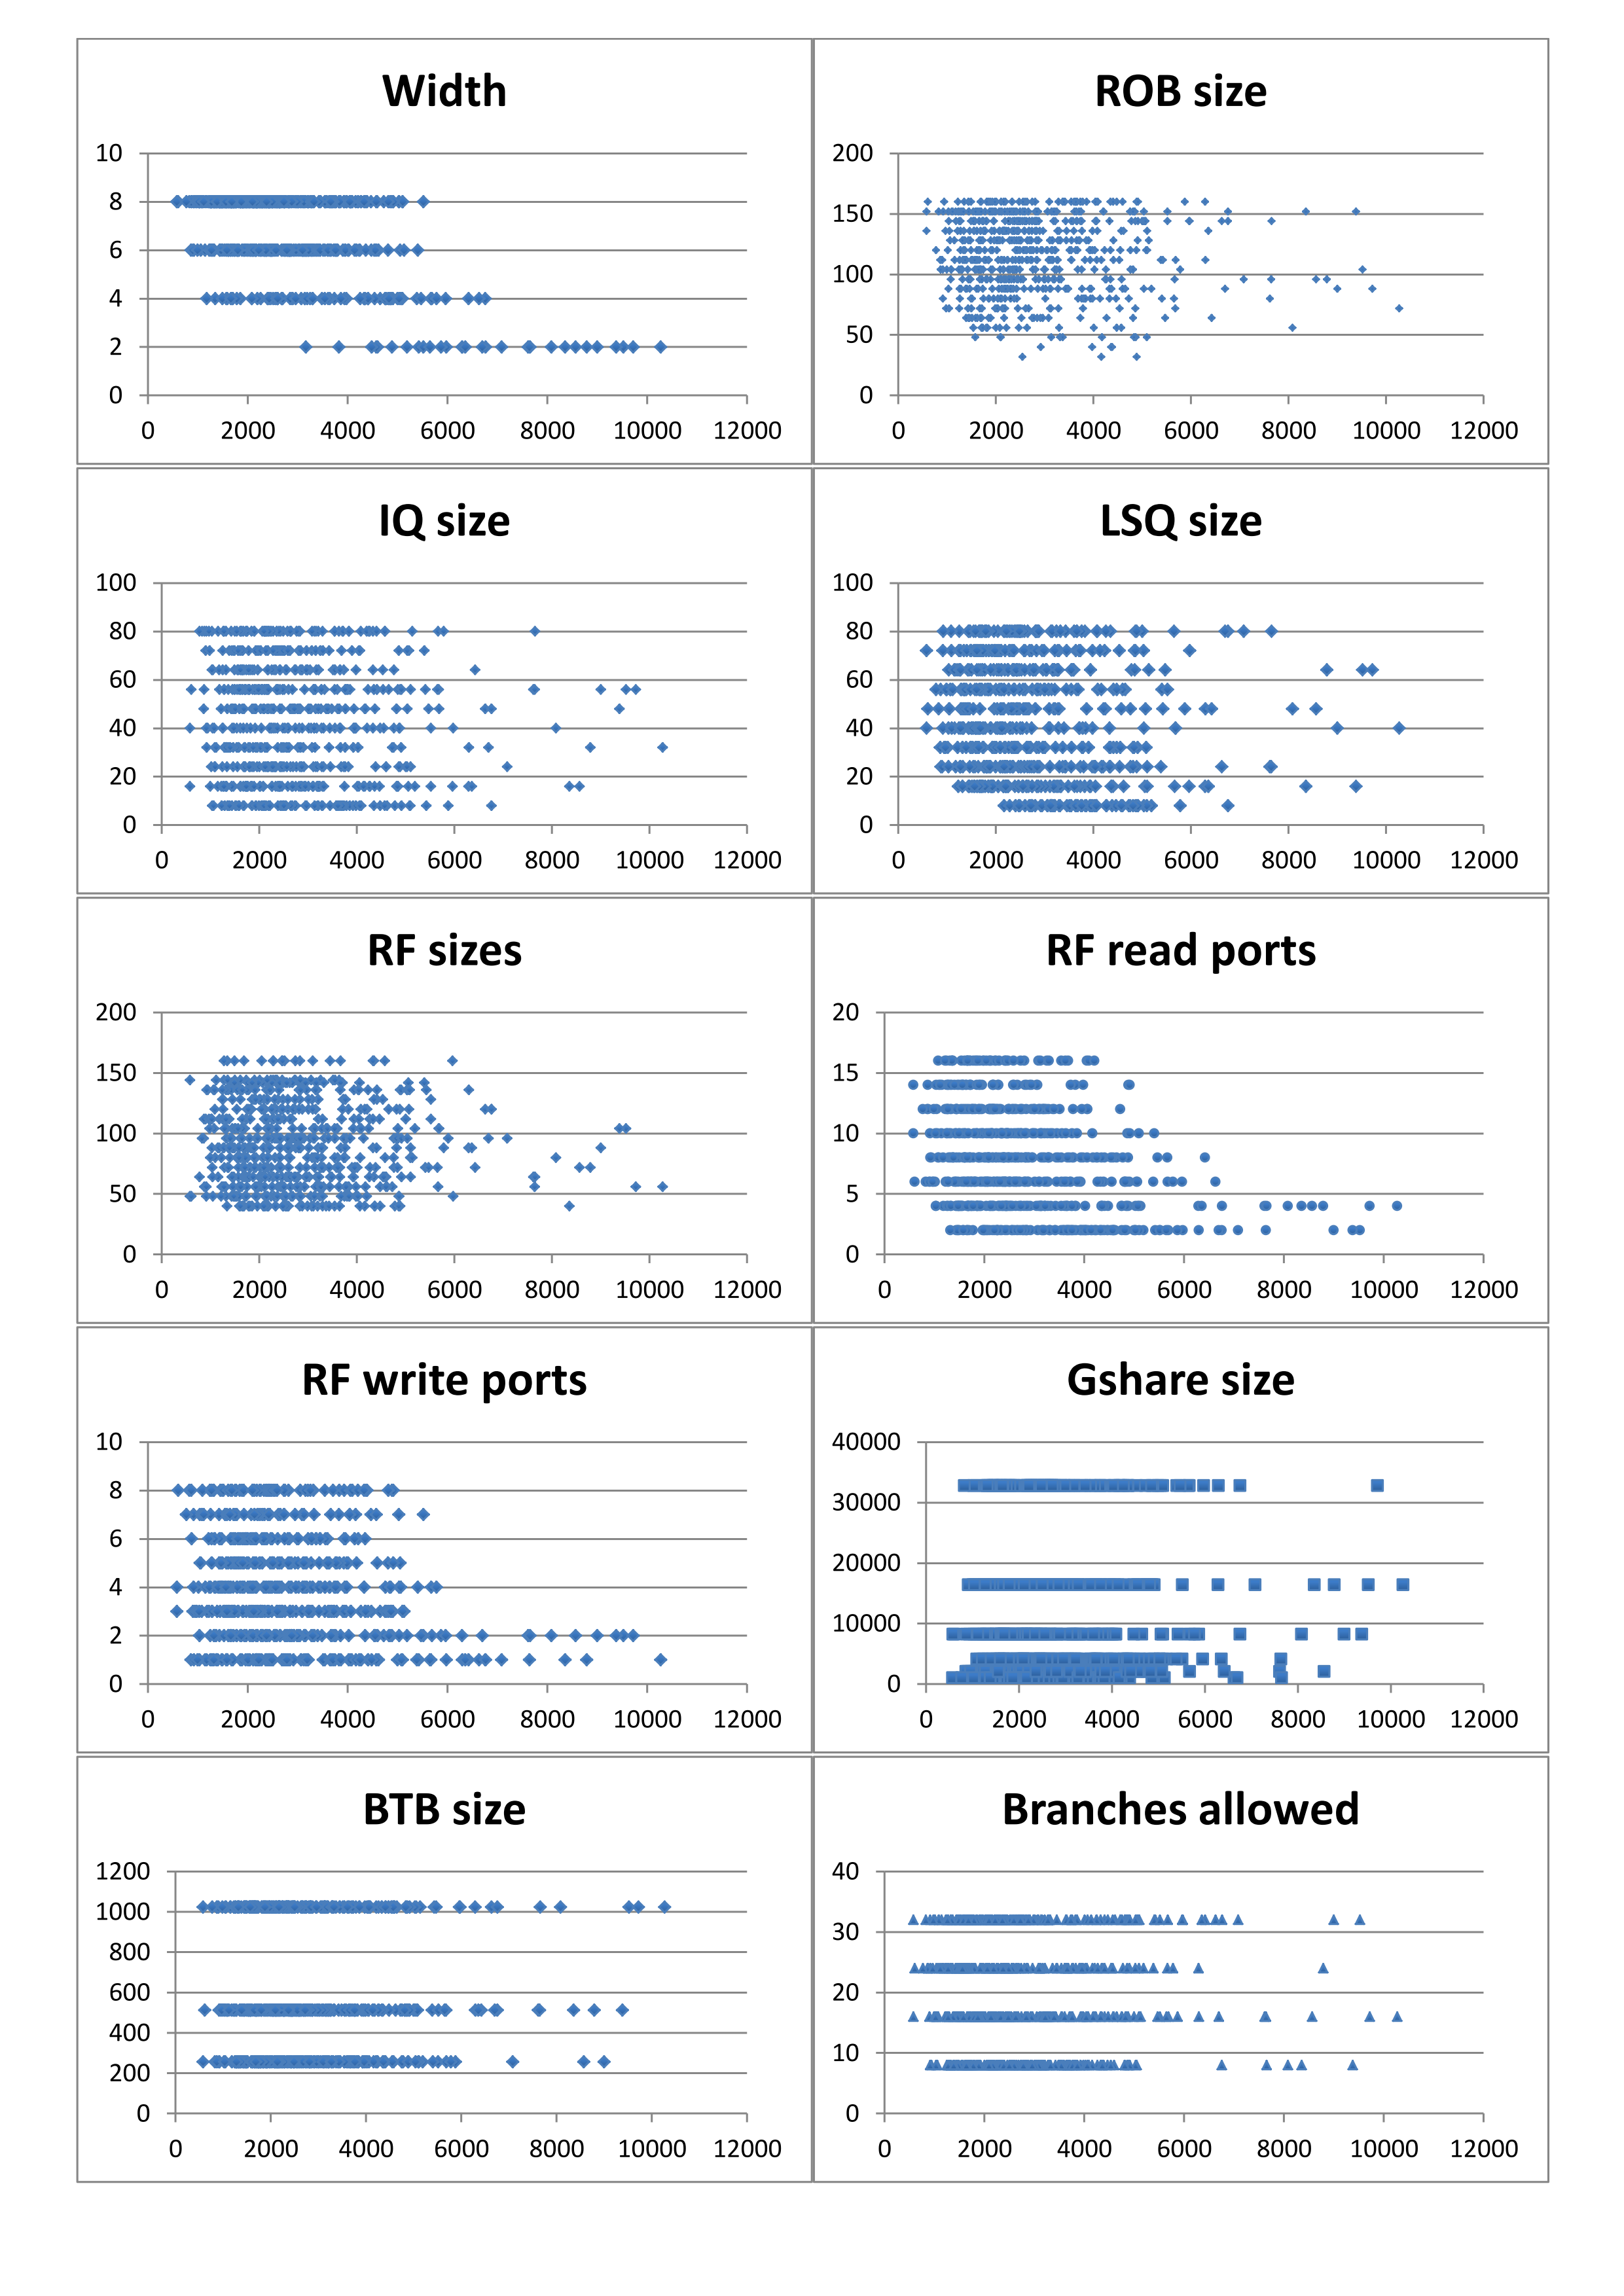
\includegraphics[height=\textheight]{graph.png}
	\caption{Plotting different features together with the target 			value may give some insights about the data distribution and the 			feature importance.}
\end{figure}

\end{document}
